\documentclass[10pt]{exam}
\usepackage[icp]{template-for-exam}
\usepackage{graphicx}

\title{Periodic Table Basics}
\author{Rohrbach}
\date{\today}

\begin{document}
\maketitle

\noindent
Every periodic table should have the following information on it: the atomic number, the element symbol, and the atomic mass.

\begin{center}
  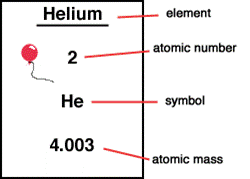
\includegraphics[width=4cm]{ptable.png}
\end{center}


\begin{questions}

\question
  Look at a periodic table. What do you notice about the atomic numbers as you read from left to right? 
  \vs

\question
  Atomic masses are usually written with decimals or in parentheses.  What do you notice about the atomic masses are you read from left to right on the periodic table?
  \vs

\question
  Listed below are elements you will find on the periodic table.  Find them and write the missing information in the boxes.

\begin{center}
    \renewcommand{\arraystretch}{2}
  
    \begin{tabular}{|c|p{15em}|c|c|c|}
      \hline
      \bf Symbol         &
      \bf Element Name   &
      \bf Atomic Number  &
      \bf Atomic Mass       \\\hline
      H	 &          &    &  \\\hline		
      He &          &    &  \\\hline		
         & Lithium  &    &  \\\hline				
         & Aluminum &    &  \\\hline		
         &          & 47 &  \\\hline		
         &          & 79 &  \\\hline		
         &          & 20 &  \\\hline	
      Mg &          &    &  \\\hline		
      S  &          &    &  \\\hline		
         & Chlorine &    &  \\\hline				
         & Argon    &    &  \\\hline	
      
    \end{tabular}
\end{center}

\end{questions}

\end{document}